%% ----------------------------------------------------------------
%% Thesis.tex -- MAIN FILE (the one that you compile with LaTeX)
%% ---------------------------------------------------------------- 

% Set up the document
\documentclass[a4paper, 12pt, twoside]{Thesis}  % Use the "Thesis" style, based on the ECS Thesis style by Steve Gunn
\graphicspath{{Figures/}}  % Location of the graphics files (set up for graphics to be in PDF format)

% Include any extra LaTeX packages required
\usepackage[square, numbers, comma, sort&compress]{natbib}  % Use the "Natbib" style for the references in the Bibliography
\usepackage{verbatim}  % Needed for the "comment" environment to make LaTeX comments
\usepackage{vector}  % Allows "\bvec{}" and "\buvec{}" for "blackboard" style bold vectors in maths
\usepackage{textcomp}
\usepackage{tikz}
\usepackage{setspace} 
\hypersetup{urlcolor=black, colorlinks=true}  % Colours hyperlinks in blue, but this can be distracting if there are many links.
\usepackage{times}
\usepackage{missing_packages/lineno}
\linenumbers
%% ----------------------------------------------------------------
\begin{document}
\frontmatter	  % Begin Roman style (i, ii, iii, iv...) page numbering
% Set up the Title Page
\title  {Multi Segmented Image Transfer in Delay Tolerant Networks using Bandwidth Reduction Technique}
\authors  {\texorpdfstring
            {\href{pratyush.anand@st.com
}
            {Pratyush Anand}}
            {Pratyush Anand}
            }
\addresses  {\groupname\\\deptname\\\univname}  % Do not change this here, instead these must be set in the "Thesis.cls" file, please look through it instead
\date       {\today}
\subject    {}
\keywords   {}

\maketitle

%% ----------------------------------------------------------------

\setstretch{2.0}  % It is better to have smaller font and larger line spacing than the other way round

% Define the page headers using the FancyHdr package and set up for one-sided printing
\fancyhead{}  % Clears all page headers and footers
\rhead{\thepage}  % Sets the right side header to show the page number
\lhead{}  % Clears the left side page header

\pagestyle{fancy}  % Finally, use the "fancy" page style to implement the FancyHdr headers


%% ----------------------------------------------------------------
\pagestyle{empty}  % No headers or footers for the following pages

\null\vfill
% copyright page

\cleardoublepage  % copyright page ended, start a new page
%% ----------------------------------------------------------------
%% ----------------------------------------------------------------
\frontmatter	  % Begin Roman style (i, ii, iii, iv...) page numbering

%\setstretch{1.3}  % It is better to have smaller font and larger line spacing than the other way round

% Define the page headers using the FancyHdr package and set up for one-sided printing
\fancyhead{}  % Clears all page headers and footers
\rhead{\thepage}  % Sets the right side header to show the page number
\lhead{}  % Clears the left side page header

\pagestyle{plain}  % Finally, use the "fancy" page style to implement the FancyHdr headers

%% ----------------------------------------------------------------
%\setstretch{1.5}  % Reset the line-spacing to 1.3 for body text (if it has changed)

% The Acknowledgements page, for thanking everyone
\acknowledgements{
\addtocontents{toc}{\vspace{1em}}  % Add a gap in the Contents, for aesthetics

Add Ack
\\
\\
\begin{flushright}
$_{\rule[1em]{10em}{0.25pt}}$\\
Pratyush Anand\\  % This prints a line for the signature
Date:\ \ \ \ \ \ \ \ \ \ \ \ \ \ \ \ \\
\end{flushright}

}


\cleardoublepage  % End of the Acknowledgements

%% ----------------------------------------------------------------



%% ------------------------------------------------------------------------------------------------------
% Declaration Page required for the Thesis, your institution may give you a different text to place here
\begin{sloppypar}
\certificate{

\addtocontents{toc}{\vspace{1em}}  % Add a gap in the Contents, for aesthetics
This is to certify that the thesis titled
``Multi Segmented Image Transfer in Delay Tolerant Networks using Bandwidth Reduction Technique''
 being submitted by PRATYUSH ANAND, Entry Number 2010EEY7515, in partial fulfillment of the requirements for
 the award of the degree of MS(R) Part Time, in Department of Electrical Engineering, Indian Institute of 
Technology Delhi, is a bonafide record of the work carried out by him under my supervision.
The matter submitted in this dissertation has not been admitted for an award of any other degree anywhere.
\\ \\ \\
 \\
Signed:\\
\rule[1em]{25em}{0.25pt}\\  % This prints a line for the signature
Date:\\
Prof. Subrat Kar\\
Department of Electrical Engg\\
Indian Institute Of Technology Delhi\\
New Delhi-110016 India  % This prints a line to write the date
}
\end{sloppypar}
\cleardoublepage  % Declaration ended, now start a new page
%% ------------------------------------------------------------------------------------------------------


% The Abstract Page
\addtotoc{Abstract}  % Add the "Abstract" page entry to the Contents
\abstract{
For a video surveillance system, image transfer over a low bandwidth
channel has always been challenging task. Specially, if image is taken
from a live camera and it has to be transmitted over a wireless delay
tolerant network, then the task is twisted a bit more.Complexity
increases further, if we need to build a viable low cost system with a
low power solution. Such solution is only possible if we extract only
relevant information from the video frame and transmit it over the
network.This work is an attempt to frame such a low data rate image
pipeline with considerably minimal computational cost. We have reviewed
all important background subtraction algorithm with their merits and
demerits. One of the efficient background subtraction algorithm called
Visual background extractor (Vibe)has been coded in 'C' and has been
compared with another important algorithm based on texture and motion.
We have also evaluated various human detection algorithms.  We have
selected a skeleton based detection algorithm. Various skeletonization
algorithm has been compared and found that star skeleton based approach
is best suited for our pipeline. Finally we have compared our pipeline
computation time with some other detection algorithm.So overall, We are
stripping down each moving object to few pixel, mainly the skeleton
endpoints and then recognize moving object based on motion information.
\addtocontents{toc}{\vspace{1em}}  % Add a gap in the Contents, for aesthetics
}

\cleardoublepage  % Abstract ended, start a new page
%% ----------------------------------------------------------------
%% ----------------------------------------------------------------

\pagestyle{plain}  %The page style headers have been "empty" all this time, now use the "fancy" headers as defined before to bring them back


%% ----------------------------------------------------------------
\lhead{\emph{Contents}}  % Set the left side page header to "Contents"
\tableofcontents  % Write out the Table of Contents

%% ----------------------------------------------------------------
\lhead{\emph{List of Figures}}  % Set the left side page header to "List if Figures"
\listoffigures  % Write out the List of Figures


%% ----------------------------------------------------------------
%\setstretch{1.5}  % Set the line spacing to 1.5, this makes the following tables easier to read
\clearpage  % Start a new page
\lhead{\emph{Glossary}}  % Set the left side page header to "Abbreviations"
\listofsymbols{ll}  % Include a list of Abbreviations (a table of two columns)
{
% \textbf{Acronym} & \textbf{W}hat (it) \textbf{S}tands \textbf{F}or \\
\textbf{DTN} & \textbf{D}elay \textbf{T}olerant \textbf{N}etwork\\
\textbf{WSN} & \textbf{W}ireless \textbf{S}ensor \textbf{N}etwork\\
\textbf{PSNR} & \textbf{P}eak \textbf{S}ignal to \textbf{N}oise \textbf{R}atio\\
\textbf{FOV} & \textbf{F}ield \textbf{O}f \textbf{V}iew\\
\textbf{SIMD} & \textbf{S}ingle \textbf{I}nstruction  \textbf{M}ultiple \textbf{D}ata\\
\textbf{PCA} & \textbf{P}rincipal \textbf{C}omponent  \textbf{A}nalysis\\
\textbf{FG} & \textbf{F}ore \textbf{g}round\\
\textbf{BG} & \textbf{B}ack \textbf{g}round\\
\textbf{BGS} & \textbf{B}ack \textbf{g}round \textbf{S}ubtraction\\
\textbf{LBP} & \textbf{L}ocal \textbf{B}inary \textbf{P}attern\\
\textbf{GMM} & \textbf{G}ausian \textbf{M}ixture \textbf{M}odel\\
\textbf{PFinder} & \textbf{P}erson \textbf{Finder} \\ 
\textbf{Vibe} & \textbf{Vi}sual \textbf{b}ackground \textbf{e}xtractor \\
\textbf{HOG} & \textbf{H}istogram of \textbf{O}riented \textbf{G}radient \\
}



%% ----------------------------------------------------------------
\clearpage  %Start a new page

%% ----------------------------------------------------------------
\mainmatter	  % Begin normal, numeric (1,2,3...) page numbering
\pagestyle{plain}  % Return the page headers back to the "fancy" style

% Include the chapters of the thesis, as separate files
% Just uncomment the lines as you write the chapters

% Chapter 1

\chapter{Introduction} % Write in your own chapter title
\label{Chapter1}
Image transfer over a low bandwidth channel has always been challenging
task. Specially, if image is taken from a live camera and it has to be
transmitted over a wireless delay tolerant network, then the task is further
twisted. Complexity increases further, if we need to build a viable low
cost system with a low power solution. In any such solution it would be
wise to transmit information only. Yes, information!!!  Information
about image!! We need to extract information out of image and then to
send it over the network.  Information can be of various type. So, we
need to deal that what minimum information about image allows us to
reconstruct the scenario or to detect an event. We also need to look
that how can these informations be represented so that it helps in
efficient system(SW/HW) development.Most appropriate application for
above technology can be smart video surveillance network.

\section{Motivation}

Most of the existing video surveillance system is still manual. Normally
all the surveillance camera video is sent to a monitoring base station,
where it is monitored by a person or a group of person. But such
arrangement can not be full proof. So, any attempt in the direction of
its automation can be of great use in following application areas:
\begin{enumerate}
 \item  Traffic Monitoring
  \item Elderly care
  \item Security
  \item Surveillance
  \item Assembly Line Inspection
\end{enumerate}

End goal of such an intelligent system would be to offer an
automatic analysis of scene and then to infer desired information out of
it.Such a system can be lot complex because of the complexity of the
scene, specially when application is targeted for outdoor monitoring.
Sometime background of the scene can be moving, while in some
other scene ambient light can be different. Similarly can be many other
hurdles in the process of automation. But if an efficient
background detection algorithm is chosen then, these issued can be
addressed up to a lot extent.



\section{Past Work and Literature Survey}

Overall this task can broadly be divided into two categories: Extraction
of information from images \& then representation of that information
through a semantic network.

\subsection{Extraction of Semantic information from Image}

Various research have been done to extract useful information from a
moving image. The toughest part of this implementation is to find an
efficient background estimation algorithm so that moving objects can be
identified. Features such as Gradient histogram, Gray Scale (Haar),
color, texture, self-similarity and motion have been used by different
researchers. \\ 
 ~\cite{1} and many other has used color information as the feature for
estimation. But only color as feature might not be sufficient ~\cite{2}
in surveillance applications where image resolution is very low.  Adding
motion along with image intensities gives better result in moving bodies
estimation. When background color is same as foreground color then
texture features represented by local binary pattern ~\cite{3} provides
interestingly nice result. Further, features computed at a single scale
can be used to approximate feature at nearby scale. Such implementations
~\cite{4} accelerates the execution for practical applications.
There is one implementation ~\cite{5} which decides about pixel that
whether it belongs to foreground or background dynamically.

Once all moving bodies have been separated out, then only points of
their contour or centroid can be sent over network.

\subsection{Representation of Semantic information}

\section{Issues and outstanding problems}

Methods of image transmission can broadly be divided into levels as shown
in \ref{fig1}. Most of these work have been done on lower three levels.
There are only few attempts on the upper layers ~\cite{6,7}.

\begin{figure}
\begin{center}
 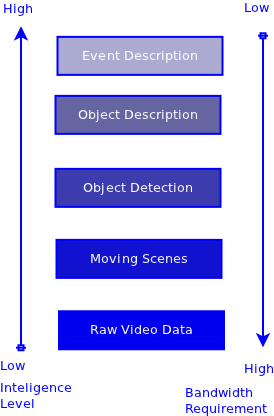
\includegraphics{../Figures/image_tr_level.png}
 % image_tr_level.png: 274x416 pixel, 72dpi, 9.67x14.68 cm, bb=0 0 274 416
 \caption{Lavel of Image Transfer}
 \label{fig1}
\end{center} 
\end{figure} 


\section{Approach}

A typical wireless sensor network can be as that of shown in figure
\ref{fig2}. Each node will have a camera, a processing engine and a
wireless transmission module. Transferring captured raw image will be
very expensive. Therefore they will be processed to
extract semantic information from it. Textual semantic information will
be transmitted over wireless media to the knowledge engine. Knowledge
engine will use ontology language such as OWL to represent these
information from different nodes. Such intelligent WSN can fit into many
important applications like security monitoring, elderly care etc.


\begin{figure}
\begin{center}
 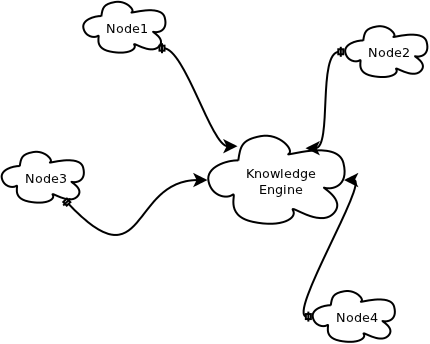
\includegraphics{../Figures/wsn.png}
 \caption{Wireless Sensor Network}
 \label{fig2}
\end{center} 
\end{figure} 


\section{Organisation of thesis}
 % Introduction

% Chapter 2

\chapter{Methodology and approach} % Write in your own chapter title
\label{Chapter2}

\section{Image analysis tools}
\indent Matlab and OpenCV~\cite{34} are two highly used image processing
tools.  Matlab comes with rich image processing and analysis libraries.
It supports most of the work discussed in chapter ~\ref{Chapter1}.
Matlab also provides interface to convert the code into a C code.
However, generated C code is normally very bulky and takes higher
execution time. OpenCV is an open source computer vision library
initiated by Intel. It is available at
http://SourceForge.net/projects/opencvlibrary. It can be used for
research or even commercial purposes. Unlike GNU Public License (GPL),
its licensing does not force that modifications to the library be made
public. \\
\indent OpenCV has been mainly developed in C and C++ on Linux platform.
However, interfaces for other scripting / programming languages such as
Python, Ruby, Java etc have also been developed. Libraries are also
available for windows, Android and Mac OS platform. OpenCV libraries
have been used in many applications since its first release in 1999.
Range of applications varies from stitching street view images together,
detecting intrusions in surveillance video, monitoring mine equipment,
helping robots navigate and pick up objects, detection of swimming pool
drowning accidents, running interactive art, checking runways for
debris, inspecting labels on products in factories, to rapid face
detection.\\
\indent OpenCV design goal is to build computer vision library with
computational efficiency which can work with real time applications. It
contains functions in almost all the area of image processing  and
computer vision like, histogram processing, morphological processing,
segmentation, detection tracking, camera calibration etc. Therefore,
selection of OpenCV libraries allows faster evaluation and development
of real embedded application.\\
\indent OpenCV libraries are also available for embedded architecture
CPUs like ARM. This allows easy porting of applications developed on x86
platform to ARM or other embedded platforms.\\
\indent Therefore, we decided to implement our image processing
algorithms in C and on Linux platform, so that it can easily be ported
from a PC to embedded environment. Wherever possible, we have used
OpenCV library.
\section{Surveillance image processing flow}
\begin{figure}[!b]
\centering
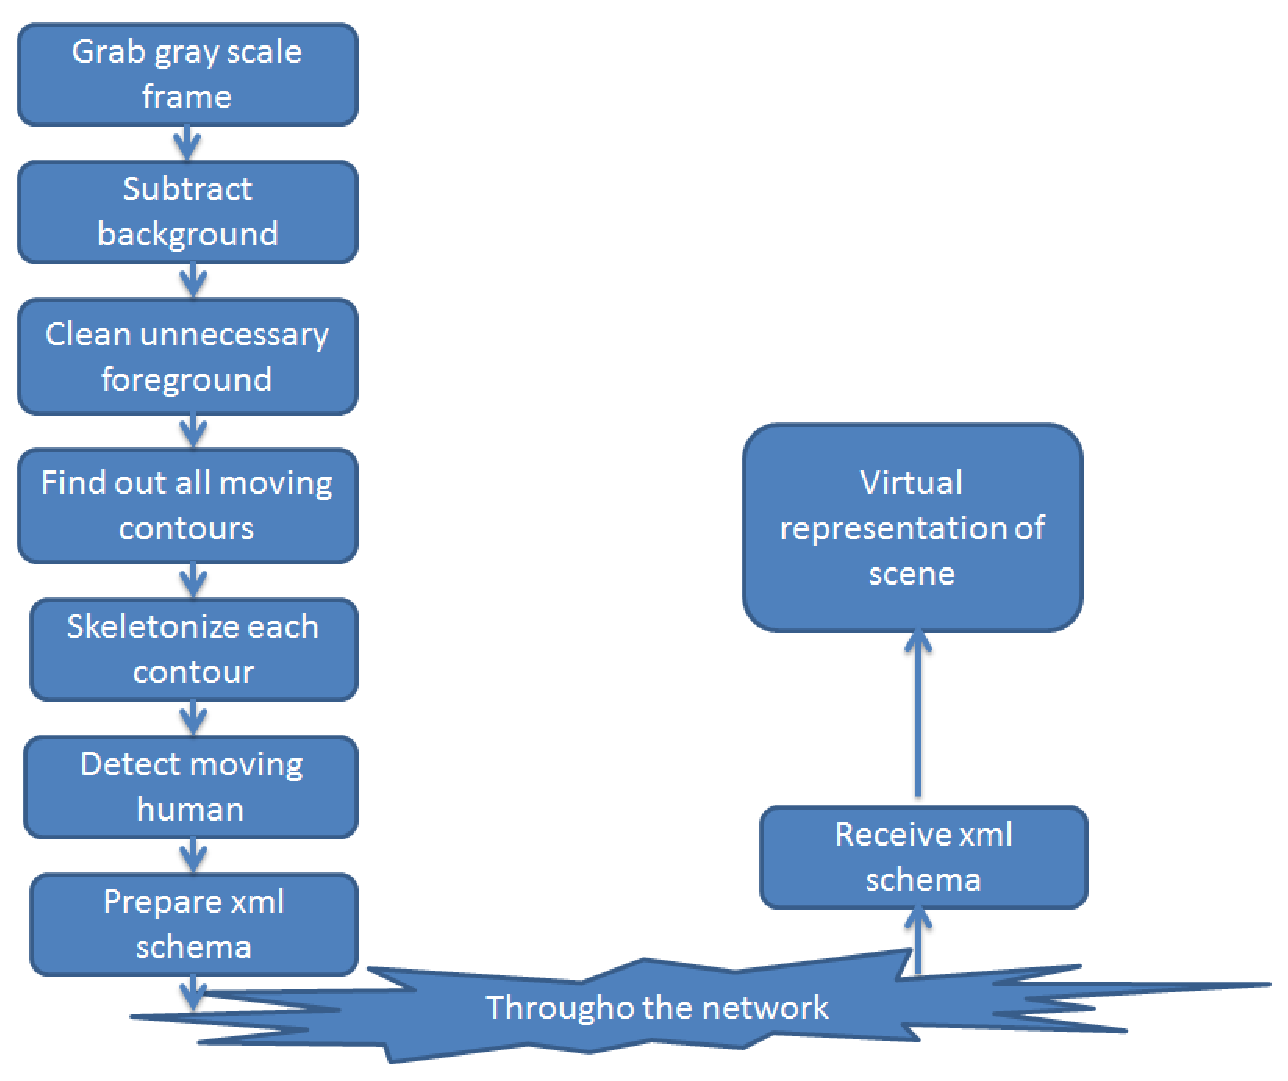
\includegraphics[height=120pt]{Figures/image_pipeline}
\caption{Low BW surveillance image application flow}
\label{image_pipeline}
\end{figure}
\indent Top level surveillance image processing flow for a low bandwidth
network is as shown in Fig.~\ref{image_pipeline}. End goal of low
bandwidth implementation would be to generate information such as human
detected, their position and the time of detection. Therefore, for above
implementation we have to decide on following items, keeping
computational efficiency and true detection for considered object as
primary objective while making any decision.\\
\begin{itemize}
\item \textbf{Background Subtraction:} Methods based on LBP by Yao et
	al.~\cite{11} have striking nice result. It works superbly with
	varied background situation like wavering tree, moving escalator
	etc. Barnich et al.~\cite{9} claim that Vibe which uses random
	sample selection also performs well in all situation and have
	extremely low computational cost. Yao et al. have provided their
	C code, however Barnich et al. have only provided an object
	library for x86 platform. Therefore we need to first code vibe
	in C and then to compare above two algorithms. We did not
	compare other algorithms like GMM, median filter etc with Vibe,
	as authors of Vibe have already done it and concluded that Vibe
	outperforms them.
\item \textbf{Detection and Tracking:} Methods based on skeleton motion
	features~\cite{32, 22, 31} seem to be computationally
	efficient. So we need to evaluate different method of
	skeletonization, suitable for motion calculation. Performance of
	detector based on such method need to be compared with other
	methods based on covariance feature with cascade of logitboost
	classifier~\cite{19}  and Haar-like features~\cite{17} for
	which C code are already available in public domain.
\item \textbf{Embedded implementation:} It is very important to see
	performance of surveillance application based on different
	algorithm on real embedded platform. ARM controller is used in
	most of the embedded multimedia applications. Therefore, it will be
	good to observe their performance with ARM controller.
\end{itemize}
\section {Evaluation of surveillance application techniques}
\subsection{Frame acquisition}
\indent OpenCV provides a way to grab frames either from a camera or
from a file. cvCaptureFromFile or cvCaptureFromCAM returns CvCapture *
struct which can further be used to query frame from either a test video
file or from camera respectively. cvQueryFrame function reads one frame
and returns its pointer. If camera's output or test video is in RGB mode
then, it need to be converted into gray scale image for further
processing. cvCvtColor function has been used to convert image from RGB
to gray scale.
\subsection{Background removal}
\indent Since background subtraction has key role in accomplishing
intended job, therefore we have compared two recently developed~\cite{3,
5} efficient background subtraction algorithm and then selected one of
them~\cite{5} in our final work.  The method described by Yao and
Odobez~\cite{3} is based on use of texture features present in Local
Binary Pattern (LBP).  LBP works well with local illumination changes,
however there can be issues in case of global illumination change. They
have carried out several improvements by using photometric invariant
color measurement and flexible weight updating for background
modes. However, our experiments says that, computationally it is very
less efficient compared to method proposed by Barnich et al.~\cite{9},
which is based on unique way of replacing background pixel value over
the time. It replaces background values for last N frames randomly.
Furthermore, it diffuses updated values to neighbouring pixels, and
again that too on random basis. We have selected method by Barnich et
al.~\cite{9} in our final application, because of its computational
efficiency while maintaining quality.  Fig.~\ref{bg_compare} shows the
comparison of execution time of these two algorithm.

\begin{figure}[!t]
\centering
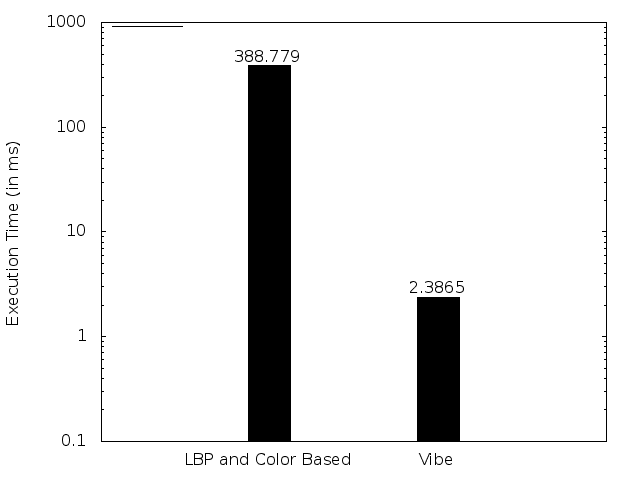
\includegraphics[height=300pt]{Figures/bg_compare}
\caption{Background subtraction average execution time of~\cite{11}
and~\cite{9}. This timing was observed with a x86 system having DMIPS =
800.}
\label{bg_compare}
\end{figure}
\subsection{Noise removal}
\indent None of the background subtraction algorithm allows pure
foreground extraction. There would always be several noise objects in the
extracted image. These are cleaned by morphological erosion operation
(cvErode) followed by dilation (cvDilate) operation. Further all moving
contours are separated out by using OpenCV library function
cvFindContours. This function provides us boundary point of individual
moving object.
\subsection{Skeletonization techniques}
\indent Image skeletons are points on the image, which are equidistant
to their boundaries.  Skeleton is a very effective way to represent
shape of an object.  Shape analysis of an object further leads to
identification of object.  Skeletonization is a process of thinning
object image by maintaining its topology. There are several mathematical
definitions to do this job. We have evaluated different skeletonization
techniques, with their merits and demerits for the suitability to our
requirement.
\begin{itemize}
\item \textbf{Contour skeleton:} When image of an object is represented by
	a single color say black, it is called silhouette. Outer boundary
	points of silhouette connected together is called contour of
	that object. Contour gives idea about global shape of an object.
	cvFindContours gives us all boundary points of a silhouette.
	However, we can analyze the shape even with lower number of
	points. cvApproxPoly can further be used to approximate it into
	polygon. Vertices of this polygon connected together gives an
	idea about outer shape of the object. An example of such
	skeleton has been shown in Fig.~\ref{skeletons}.A.

\begin{figure}[!t]
\centering
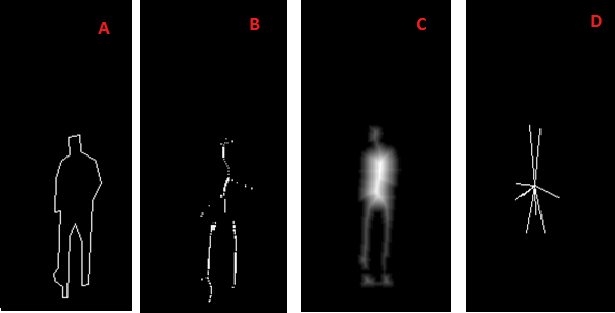
\includegraphics[height=220pt]{Figures/skeletons}
\caption{Skeleton obtained by different methods.\\
	\textbf{A.} Contour skeleton\\
	\textbf{B.} Morphological skeleton\\
	\textbf{C.} Distance transform skeleton\\
	\textbf{D.} Star skeleton}
\label{skeletons}
\end{figure}
\item \textbf{Morphological skeleton:} Morphology is a mathematical
	technique for analysis of structure of any geometry. It was
	mainly defined for the analysis of binary images. Basically, an
	image is probed with a pre-defined shape which is called
	structuring element. Gonzalez and Woods have provided
	a set of morphological operations in their book Digital image
	processing~\cite{35}, where they have defined morphological
	skeletonization as follows:
	\begin{equation}
	\begin{aligned}
		S(A) &= \Sigma ^K _{k = 0} S_k(A) \label{morph_skel}\\
	\mathrm{where} \hspace{5 mm} S_k(A) &= (A \ominus kB) - (A \ominus kB) \circ B \\
			  k &= max \{ K | (A \ominus kB) \neq \phi\}
	\end{aligned}
	\end{equation}
Translating Eqn~\ref{morph_skel} into C code: \par
\fbox{\parbox{\textwidth}{%
	do \\
	\{\\
	\hspace*{1 in}cvErode(img, eroded, element, 1);\\
	\hspace*{1 in}cvDilate(eroded, temp, element, 1);\\
	\hspace*{1 in}cvSub(img, temp, temp, NULL);\\
	\hspace*{1 in}cvOr(skel, temp, skel, NULL);\\
	\hspace*{1 in}cvCopy(eroded, img);\\
	\hspace*{1 in}done = (cvCountNonZero(img) == 0);\\
	\} while (!done);
}} \par
\indent An example of skeleton obtained by morphological method has been
shown in Fig.~\ref{skeletons}.B.
\item \textbf{Skeleton by distance transform:} Distance transform of an
	input image is obtained by creating a new image where pixels are
	set to a value equal to the distance to the nearest zero value
	pixel in input image. We have seen that the contour skeleton
	provided outer shape of the object, where as distance transform
	method provides internal orientation of object. OpenCV provides
	a function cvDistTransform, which can be used to build a
	distance transformed image. An example of skeleton obtained by
	distance transform method has been shown in
	Fig.~\ref{skeletons}.C.
\item \textbf{Star Skeleton:} In this method we plot distance of each
	boundary point from the centroid and then use peaks of the curve
	as skeleton point.
\begin{itemize}
\item Centroid of each object is found out using following
	Eqn~\ref{centroid_calc}.
	\begin{eqnarray}
	C_x = {1 \over N} \Sigma ^N _{i = 1} X_i \label{centroid_calc}
\nonumber \\
	C_y = {1 \over N} \Sigma ^N _{i = 1} Y_i 
	\end{eqnarray}
Here X$_i$ and Y$_i$ are (X,Y) co-ordinates of i$_{th}$ point on the contour
boundary.
\item Distance d$_i$ is calculated between centroid and each boundary
	point as follows. This calculated distance vector are stored in a
	CvMat array.
	\begin{equation}
	d_i = \sqrt{(C_x - X_i)^2 + (C_y - Y_i)^2} \label{dist_calc}
	\end{equation}

\begin{figure}[!t]
\centering
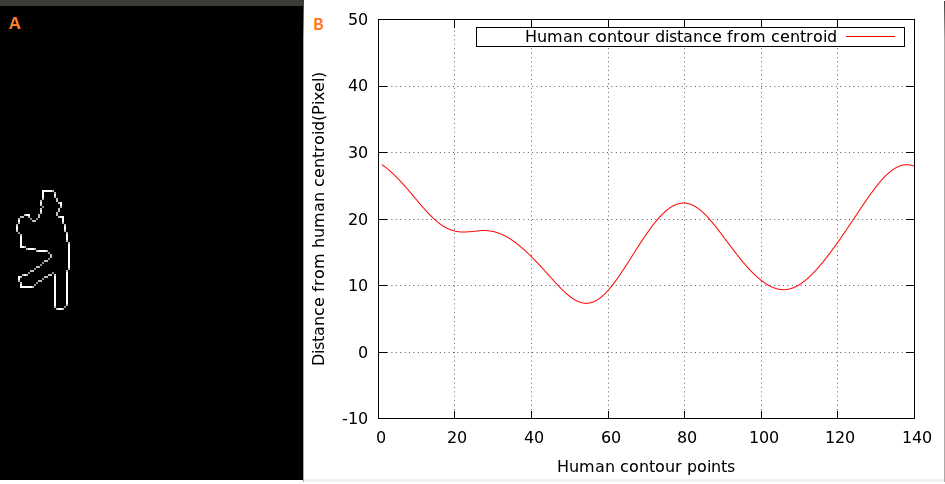
\includegraphics[height=200pt]{Figures/distance}
\caption{Distance plot of human contour points from its centroid}
\label{distance}
\end{figure}
\item Distance vector array is smoothed to remove noise peaks using
	cvSmooth. If these distances are plotted then it looks like
	Fig.~\ref{distance}. Now local maxima of distance vector is
	calculated by finding zero crossing of difference vectors. These
	local maxima provides a star form of skeleton centered at
	centroid of the object. A typical star skeleton has been shown
	in Fig.~\ref{skeletons}.C.
\end{itemize}
\end{itemize}
\subsection{Human detection methods}
\indent We have evaluated three methods of human detection technique mainly on the
basis of their computation efficiency.
\begin{itemize}
\item \textbf{Detection using covariance features:} We have used method
	implemented by Yao et al. ~\cite{19}. We have selected this
	method, because it has been widely referenced and also the
	source(C code) is available in public domain.
\item \textbf{Detection using Haar-like features:} We have evaluated
	work by Viola et al.~\cite{16, 17} which uses Haar-like
	features for human detection. Again, reason to evaluate this
	algorithm was same, that it has been widely discussed and
	referenced.
\item \textbf{Detection using skeleton motion features:} We have
	evaluated this method as it seems to be computationally very
	efficient.  We have done our own implementation in C to evaluate
	this method.  Human motion can be represented suitably by
	movement of legs. So, we use star skeletonization method which
	seems best suitable for human leg motion analysis. We have seen
	that star skeletonization gives us skeleton points in form of peak
	distance from centroid. However, some of these peak points are
	not of our interest. In our algorithm, we are using two most relevant
	peaks which are nearest to each bottom corner of bounding box of
	contour respectively. Only these two peaks along with centroid
	give us sufficient information to distinguish human from
	human, vehicle or animal etc.\\
\indent For human subjects, the two peaks correspond to the two legs of
human. For vehicles, the peaks correspond to the two extrema points of
lower portion of back and front.  When it is an animal, the peaks
correspond to front and back leg of animal.\\
\item Let P$_1$(X$_1$, Y$_1$), P$_2$(X$_2$, Y$_2$) and C(C$_x$, C$_y$)
are two peaks nearest to bottom right and bottom left corner and
centroid respectively. Let $\theta$ is the angle between the line
segments P$_1$C and P$_2$C, then $\theta$ can be calculated as
follows.\\
%
	\begin{equation}
	\theta = tan^{-1}[(Y_2 - C_y) / (X_2 - C_x)] \\ - tan^{-1}[(Y_1 - C_y) / (X_1 - C_x)]
	\end{equation}
%
\indent If variation of $\theta$ is plotted in respective frames for
human and vehicle then the resultant plot is as shown in
Fig.\ref{angle_plot}.  The observations from this plot is that for a
human subject, angle variation pattern is repeatable, and it is zero for
almost at regular intervals.  For vehicle, it is constant. The
experiment with images containing animal is yet to be done. For images
with animals in it, there are variations with repeatable patterns but
which never touch zero.  These criterion can be the basis to identify an
object, and to decide whether it is a human,vehicle or animal.

\begin{figure}[!t]
\centering
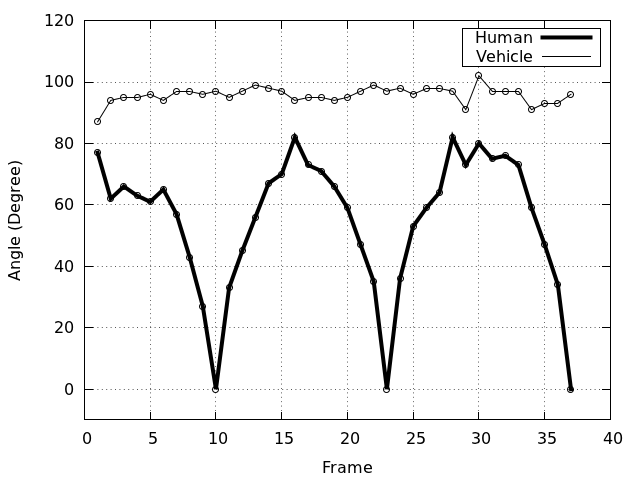
\includegraphics[height=300pt]{Figures/angle_plot}
\caption{Plot of variation of angle $\theta$ with frame number for human and
vehicle.}
\label{angle_plot}
\end{figure}
\item Every new object which comes into the field of view is tracked and
	value of (C$_x$, C$_y$), $\theta$ in each frame is stored. 
\begin{itemize} 
\item We track value of $\theta$ until it goes to zero three times.
\item Now we consider $\theta$ values between first and second zero as
vector T$_1$ and $\theta$ values between second and third zero as vector
T$_2$.
\item We find mean m$_1$ and m$_2$ of vector T$_1$ and T$_2$ respectively.
\item If n is the length of vector T$_1$ then, we calculate correlation
value (r) between these two vectors to find similarities as follows.
	\begin{equation}
	r = {{\Sigma ^n _{i = 1}(T_{1i} - m_1) . (T_{2i} - m_2)}
\over {\sqrt {\Sigma ^n _{i = 1} (T_{1i} - m_1)^2 . \Sigma ^n _{i = 1} (T_{2i}
- m_2)^2}}}
	\end{equation}
\item If correlation value is greater than a threshold value TH$_1$,
then we conclude that it is a human.
\end{itemize} 
\end{itemize} 
 %methodology and approach

% Chapter 3

\chapter{Embedded Implementation} % Write in your own chapter title
\label{Chapter3}
We have done evaluation of embedded solution of our implementation on
the basis of following:
\begin{itemize}
	\item \textbf{Low cost:} It is very important for any mass
		market product.
	\item \textbf{Low power:} Reducing energy consumption is a
		movement and is necessary for a greener world.
		Technically also it is very important for a prolonged
		battery life.
	\item \textbf{Computational power:} Selected platform must
		provide sufficient computational power to perform
		needed software operations.
	\item \textbf{Rapid software development:} Today lot of software
		is available in every domain of technology by open source
		community. Platform must be developed by considering
		re-usability of available software in public domain.
\end{itemize}
\section {Hardware Evaluation}
\indent Most of the commercial embedded systems uses following CPUs.
\begin{itemize}
	\item \textbf{MIPS:} The microprocessor without interlocked
		pipeline stages(MIPS) is based on reduced instruction
		set computer(RISC) architecture. It has been used in
		embedded products mainly for gaming and networking. Many
		operating system like Windows CE, QNX and Linux etc
		supports this architecture.
	\item \textbf{AVR32:} AVR is also a 32 bit RISC architecture CPU
		designed by Atmel. It is suited for low power and high
		code density applications.  It is also supported by
		Linux. Further, it supports hardware accelerator for
		JAVA byte code.
	\item \textbf{PPC:} Power performance PC, known as PowerPC is
		also a RISC architecture CPU. It is very popular in
		automotive, defence, networking market. However, it is not
		suitable for low power applications. It is also
		supported by Linux.
	\item \textbf{Atom:} Atom is ann ultra low voltage x86
		architecture from Intel. It is also very power
		efficient. It has been used in many notebook and mobile
		phone applications. Further, well supported by many
		operating system including Linux.
	\item \textbf{ARM:} Advance RISC machine (ARM) is again a RISC
		architecture based CPU. As of now, it is the most
		popular CPU having embedded CPU market share of more
		than two third. It is available in both 32 bit and 64
		bit versions. It has been used in product ranging from
		notebook, mobile phones, gaming devices, networking
		devices, low power storage server to almost all the
		domain of embedded applications. It is also supported by
		various operating systems including Linux.
\end{itemize}
We decided to use ARM based SOC by looking its advantages of low power
and strong support base. There are various evaluation boards available
in the market by different vendors having ARM CPUs. Few examples, BCM
family from Broadcom, SPEAr13xx family from STMicroelectronics, OMAP,
AM335x, Davinci families from Texas instruments, Tegra family from
Nvidia, Exynos family from samsung, Kirkwood, Orion5x families from
Marvel etc. Out of all these, BeagleBoard and BeagleBone based on TI
OMAP and AM335x SOCs respectively and Raspberry pi based on Broadcom
BCM2835 SOC are very popular among educational hobbyist. Both of these
boards are available with ARM ubuntu support. Raspberry pi has ARM11
core which is ARMv6 and Beagle has Cortex A8 which is ARMv7. Since we
wanted to evaluate performance of selected algorithms at a low end CPU,
therefore we carried our experiments with Raspberry pi.
\section {Software Evaluation}
\indent Developing a complete code from scratch and without using any OS
or with a very light weight kernel will have advantages in terms of boot
and execution time. However, code development would be very slow. Further,
all evaluated applications including our own developed use
OpenCV library, therefore we looked for the operating systems which
supports OpenCV. There are only two options for embedded platforms,
Windows CE and Linux. Both windows CE and Linux supports ARM
architecture, but windows CE is not free while Linux is open source.
Development over Linux has several other advantages:
\begin{itemize}
	\item Applications are portable from one architecture to
		another. Which means an applications developed on x86
		platform must also work on ARM platform.
	\item Lot of other people are working with it, so a strong
		support.
	\item Code can easily be reused by next developer.
	\item Code debugging is easier.
\end{itemize}
\section {Component of embedded Linux software}
In this section we describe about the necessary tools and software
components that we need to use / develop for complete application.
\subsection {Compiler}
\indent We use native GNU C Compiler (GCC) when code has to be executed
on x86 platform. However, we can not use the same GCC compiler at x86 if
code has to be executed on another architecture say ARM. In such case we
need a cross compiler. This cross compiler is an executable binary which
executes itself at native platform (x86) but, produces another
binary which is executable at target platform (ARM).\\
\indent Preparing a cross compiler from scratch is a tedious job. One
will need source of Linux kernel, binutils, glibc and GCC. Further,
these different sources are released independently and finding a
compatible version is another challenge. However, in most of the cases
we do not need to go through these steps. A ready to use cross toolchain
for ARM and other target is already available in the public domain.\\
\indent If we already have target ready with Linux bootable binaries,
then we can even avoid using cross compiler at all. Now a native GCC is
also available for ARM which can be used to compile Linux Kernel as well
as applications. However, compilation time of Linux kernel with the
native compiler is quite huge and therefore, its use is not preferred.
\subsection {BootROM}
\indent An ARM architecture system boots either from 0x00000000 or from
0xFFFF0000 depending on default vector mode of SOC as low vectored or
high vectored respectively. It is necessary to have a valid code at
default boot location. Normally, most of the SOCs provide hard fixed
code lying in ROM at reset boot location. This piece of software is
known as BootROM. However, there are SOCs which allows to connect
external ROM/Flash memories at reset boot address. \\
\indent This minimal software allows the system to load bigger binaries
from different sources. SOCs are available with boot from USB device, SD
card, NOR / NAND Flash, PCIe device etc. A particular boot mode is
selected using combination of user GPIO pins. In all the boot mode,
common practice is used as follows. BootROM gets first and second level
boot code from external host / device and executes it in SOC's internal
SRAM and external DRAM respectively. Depending on the boot mode ,
bootROM code behaves either as master or slave.\\
\indent For example, bootROM works as slave in USB device mode. USB
device port of SOC is connected to the USB host port of PC. A custom
driver at PC enumerates this bootROM device. BootROM USB device normally
waits for an executable binary from host PC in a loop. New binary is
executed as soon as it is received.\\
\indent BootROM works as master in SD boot mode. It initializes SD
controller and then looks for predefined executables in SD device. If
a valid executable is found, then it is executed.
\subsection {First level boot loader}
\indent RAM is an important part of embedded system which is needed as
run time memory. Normally SOC is designed with some amount of internal
SRAM. SRAM memory is directly accessible and no software initialization
is needed. However, it is very costly. Therefore, connecting even
external SRAM for extra needed RAM is not advised. When an embedded
software executable needs bigger amount of main memory such as in Mega
Bytes, then use of DRAM is preferred. However, DRAM is not directly
accessible by the CPU. First level boot loader has a role to
initialize DRAM controller, so that memory is transparently visible to
CPU. In some cases, first level boot loader itself loads second level
boot loader, while in some other control is passed back to bootROM which
loads second level boot loader. There can be few light weight system
where, second level boot loader is avoided and kernel is directly
loaded.
\subsection {Second level boot loader}
\indent Second level boot loader has following responsibilities:
\begin{itemize}
	\item Provides a debug console till kernel initializes
		console driver. Normally UART is used as initial debug
		console in an embedded environment.
	\item Initializes few more hardware needed for kernel booting.
	\item Provides boot arguments to the kernel. These arguments
		allow kernel and file system to load in a particular
		specification.
	\item Brings kernel to the main memory.
	\item Transfers control to kernel for further execution.
\end{itemize}
\subsection {Kernel}
\indent Kernel is the core of software system. It has following primary
responsibilities:
\begin{itemize}
	\item It initializes all the needed hardware resources like
		cpu, camera, USB, DMA, memory, network controller,
		console and other various input and output devices.
		Linux has huge advantage here. It supports most of the
		hardware available in the market.
	\item It manages cache sync when main memory is used by more
		than one master such as DMA and CPU.
	\item Kernel controls the execution of different task. It
		schedules them on the basis of priorities of the task
		and chosen scheduling algorithm.
	\item Kernel program as well as user space application need huge
		amount of dynamic memory. These memories are allocated
		and freed at run time. It is also very important that
		they are well protected and any illegal access is
		appropriately reported. Kernel takes care of all these
		by proper memory management, allocation and
		deallocation.
	\item It supports various user space file system.
	\item Finally it calls first user space function called init.
\end{itemize}
\subsection {Root filesystem}
\indent	File system defines the way a file can be stored in the memory.
Root file system is the primary file system where root directory is
located. All other file system can be mounted within a sub-directly of
this root file system. Linux kernel supports file system like etx2,
ext3, ext4, ntfs , fat32 etc. However, embedded Linxu uses cramfs,
jffs2, yaffs2 which are more suitable for flash. Network File System
(NFS) is also supported by Linux which is very useful during kernel
debug phase.
\section {Application execution at Raspberry pi}
BootROM of Raspberry pi provides boot from SD card. Its boot process can
be summarized as under:
\begin{itemize}
	\item It initializes SD controller and looks for any connected
		SD device.
	\item If a device is found, it looks for a valid FAT32 file
		system.
	\item Then it searches for $bootcode.bin$, which is the first
		level boot loader. This binary file is copied to L2
		cache. L2 cache is treated here as SRAM. Execution of
		this binary does the job of SDRAM initialization.
	\item Once SDRAM is available, $start.elf$ is copied from SD
		disk to SDRAM and is executed from there. $start.elf$
		functions as second level boot code. It reads
		$cmdline.txt$ and $config.txt$ and passes boot arguments to
		kernel accordingly.
	\item Second level boot loader copies $kernel.img$ at 0x8000.
	\item Till this point everything was executed at GPU of BCM2837.
	\item $kernel.img$, is the first binary that runs on the ARM
		processor.
	\item When kernel is booted, it looks for ext4 root file system at
		the second partition of SD card. If a valid root file
		system is found, it executes $/sbin/init$ , the first user
		process.
\end{itemize}
\subsection {Raspberry pi kernel compilation}
\begin{itemize}
	\item RPI kernel git repository is cloned.\par
		\framebox[1.1\width]{git clone https://github.com/raspberrypi/linux.git} \par
	\item Working tag / branch checked out.\par
		\framebox[1.1\width]{git checkout -b rpi\_working origin/rpi-3.6.y} \par
	\item Following default configurations are available in
		$arch/arm/configs$ directory for RPI platform. 
		\begin{itemize}
			\item bcmrpi\_cutdown\_defconfig
			\item bcmrpi\_defconfig
			\item bcmrpi\_emergency\_defconfig
			\item bcmrpi\_quick\_defconfig
		\end{itemize}
		Cut down configuration is selected for a lighter
		kernel.\par
		\framebox[1.1\width]{make ARCH=arm CROSS\_COMPILE=arm-linux-gnueabi- bcmrpi\_cutdown\_defconfig} \par
		$arm-linux-gnueabi-$ is ARM cross compiler provided by Ubuntu Linux package.  
	\item Above $make$ prepares a $./config$ for kernel configuration.
		This default configuration can be modified further by
		$menuconfig$ operation, if needed.\par
		\framebox[1.1\width]{make ARCH=arm CROSS\_COMPILE=arm-linux-gnueabi- menuconfig } \par
	\item Then the kernel image is prepared.\par
		\framebox[1.1\width]{make ARCH=arm CROSS\_COMPILE=arm-linux-gnueabi- } \par
		Two kernel images are prepared in $arch/arm/boot$ directory by
		above command. Kernel image with name $Image$ is
		uncompressed and with name $zImage$ is compressed. RPI
		boot loader $start.elf$ expects a uncompressed kernel
		image. Therefore copy $arch/arm/boot/Image$ to SD card.
		If host PC has multiple CPU then -j option can be used
		for faster compilation. Following command will use four
		CPUs in parallel for compilation.\par
		\framebox[1.1\width]{make ARCH=arm CROSS\_COMPILE=arm-linux-gnueabi- j4 } \par
	\item If a driver is selected to be loaded as module at run time
		then, modules can be prepared as follows:\par
		\framebox[1.1\width]{make ARCH=arm CROSS\_COMPILE=arm-linux-gnueabi- modules} \par
		Install all modules to $/lib/modlues/$ directory of ext4
		partition of SD card.\par
		\fbox{\parbox{\textwidth}{%
				make ARCH=arm CROSS\_COMPILE=arm-linux-gnueabi- \\
				\hspace*{40 mm}INSTALL\_MOD\_PATH=/tmp/ modules\_install\\
				cp -r /tmp/lib/modules/* /mnt/lib/modules/
		}} \par
		Here, ext4 partition of SD card has been mounted to $/mnt$.
\end{itemize}
 %results and conclusion

% Chapter 4
\chapter{Results and conclusion} % Write in your own chapter title
\label{Chapter4}
\indent In this section we discuss results of different evaluations and
also how does our implementation compares with others. We also draw
conclusions and future works to be done.
\section{Results}
\indent From Fig.~\ref{bg_compare}, we infer that Vibe is
computationally very efficient compared to other.  We target human
detection based on its skeleton motion. We have seen different skeleton
output in Fig.~\ref{skeletons}. We have also seen that star skeleton
provides a simple way for leg motion analysis. Therefore we have used
Vibe~\cite{9} as background subtracter and \textbf{Skel}etonized
\textbf{M}otion \textbf{A}nalysis (SKELMOT) based on star skeleton for
object detection in our final implementation.\\
\indent We conclude that with our implementation, system is able to
detect a moving person after it's 3 steps move.
Fig.~\ref{pipeline_images} shows output images at different stages of
pipeline.\\

\begin{figure}[!b]
\centering
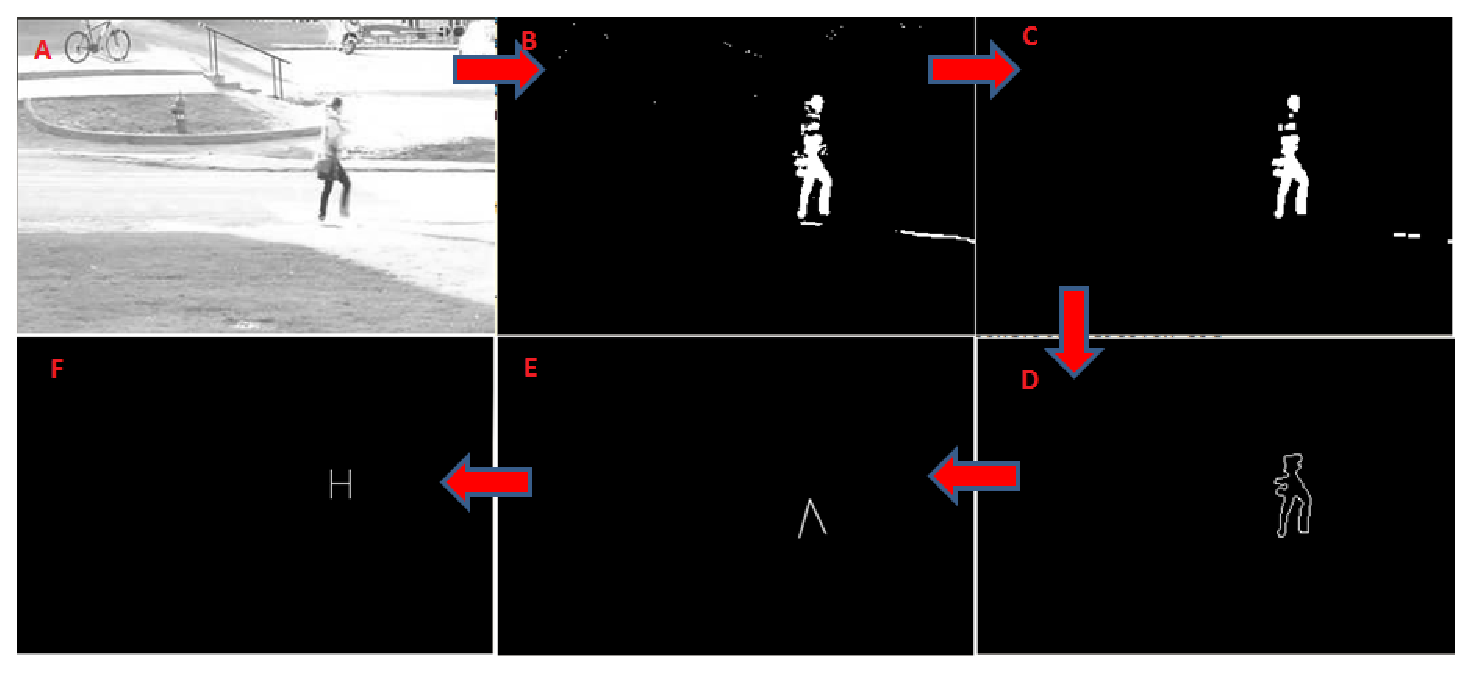
\includegraphics[height=200pt]{Figures/pipeline_images}
\caption{Images at different stages of implementation. (From top left in
clockwise order) \textbf{a.} Gray Scale input frame
\textbf{b.}Foreground extracted image using Vibe \textbf{c.} Cleaned
image \textbf{d.} Contour of moving object \textbf{e.} Plot of 3 points
of interest, centroid and two distance peaks nearer to bottom left and
bottom right corner of bounding box \textbf{f.} Virtual representation
of scene} 
\label{pipeline_images}
\end{figure}
\indent We have also done experiments with negative images like a person
moving on bicycle, or a vehicle moving on road. SKELMOT is successfully able
to discriminate between these objects. Fig.\ref{negative_inputs} shows
how it rejects moving vehicle and bicycle and  does not detect them as
human.\\

\begin{figure}[!b]
\centering
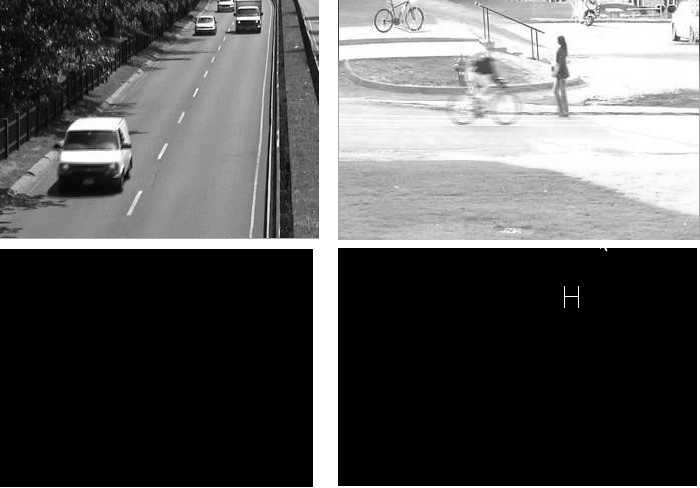
\includegraphics[height=300pt]{Figures/negative_inputs}
\caption{Input and output of pipeline in case of negative images}
\label{negative_inputs}
\end{figure}

\indent We have implemented and executed SKELMOT, Haar-like~\cite{19} and
covariance~\cite{19} feature based detection algorithm on both x86
desktop computer and embedded ARM platform. Comparison of execution time
has been shown in Fig.\ref{pipeline_execution_time}. It shows a
definite improvement in execution speed of SKELMOT over HAAR and covariance
feature based approach.  SKELMOT takes just 3.6 ms on the average, while
HAAR and covariance feature based algorithm take around 20 ms and 248 ms
respectively per frame on x86 platform having DMIPS = 800. Comparison of
timing on ARM platform with DMIPS = 44 shows that SKELMOT takes 182 ms
on the average, while HAAR and covariance feature based algorithm take
around 942 ms and 4.65 s respectively per frame.  \\
\begin{figure}[!h]
\centering
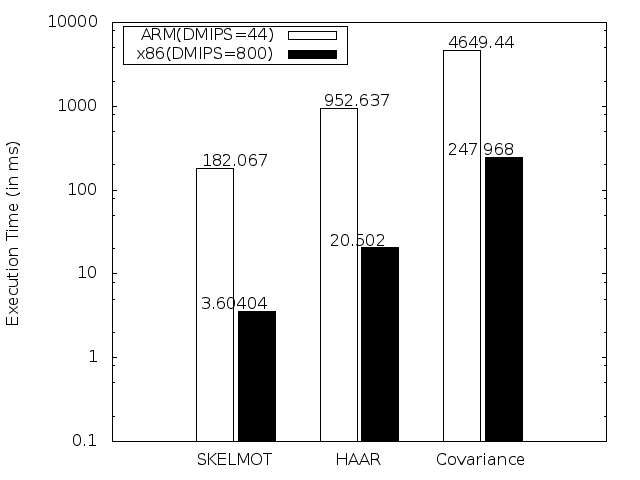
\includegraphics[scale=0.30]{Figures/pipeline_execution_time}
\caption{Execution time of evaluated algorithms on ARM and x86
platform}
\label{pipeline_execution_time}
\end{figure}
\section{Conclusion}
\indent We have seen that method based on covariance or Haar-liek
descriptor is very slow in comparison with skeleton motion descriptor.
Therefore, if a surveillance application requires to identify moving
person, then we might not need to use complex algorithm to get real time
performance with low cost embedded platform. By using proposed
algorithm, we can save a lot of computational power. However, if we wish
to detect human from still frame, then we need to go for other methods.
To use other methods such as haar or covariance features based
descriptor in real time environment, we recommend to implement them in
hardware. This dedicated hardware can further be used with low end
micro-controller to achieve end result.
\section{Future work}
Future work may be carried in following directions:
\begin{enumerate}
\item Test of this algorithm with real camera connected and Zigbee
network will provide good confidence to use it.
\item A research work may be initiated to see actual power saving using
such a low complexity pipeline.
\item There can be improvement in blob tracking algorithm to predict
next position on the basis of past N number of frames.
\item We have seen that low end micro-controller is not able to work with
single frame human detection algorithms. These algorithm can either run on
high performance CPU, or GPU. A work can be initiated to implement such
algorithms in hardware and then to use this hardware with low end
micro-controller. It would be interesting to see difference between power
consumption of two systems.
\item 
\end{enumerate}



 %future work

%% ----------------------------------------------------------------
\label{Bibliography}
\addtotoc{Bibliography}
\lhead{\emph{Bibliography}}  % Change the left side page header to "Bibliography"
%\bibliographystyle{ieeetr}  % Use the "unsrtnat" BibTeX style for formatting the Bibliography
\bibliographystyle{apalike}
\bibliography{Bibliography}  % The references (bibliography) information are stored in the file named "Bibliography.bib"
\cleardoublepage


\addtotoc{About the Author}
\lhead{\emph{About the Author}}
\huge\textbf{About the Author}

\begin{sloppypar}
\normalsize
Add about the author.
\end{sloppypar}


\end{document}  % The End
%% ----------------------------------------------------------------
